\section{Auswertung}
\label{sec:Auswertung}
\subsection{Elektronen im E-Feld}
\label{subsec:E-Feld}

Zunächst wird die Empfindlichkeit $D/U_d$ mithilfe einer Ausgleichsrechnung durch Python ermittelt.
Die nach \autoref{sec:Durchführung} aufgenommenen Messwerte sind in \autoref{tab:eFeldTeil1}, sowie in \autoref{fig:eFeldTeil1a} zu finden.
Zudem wird zu jedem Messsatz eine lineare Ausgleichsrechnung nach $D = a \cdot U_d + b$ durchgeführt.
Folgende Werte werden ermittelt:
\begin{align*}
    U_\text{b} = \SI{180}{\volt} :&  &a&= &(-0.5371 \pm 0.0060) \si{\centi\metre\per\volt}\\
    &  &b&= &(-2.1190 \pm 0.1182)\si{\centi\metre}\\
    \\
    U_\text{b} = \SI{240}{\volt}:& &a&= &(-0.7039 \pm 0.0048) \si{\centi\metre\per\volt}\\
    & &b&= &(-1.6669 \pm 0.0948) \si{\centi\metre}\\
    \\
    U_\text{b} = \SI{275}{\volt}:& &a&= &(-0.7806 \pm 0.0041) \si{\centi\metre\per\volt}\\
    & &b&= &(0.0258 \pm 0.0819) \si{\centi\metre} \\
    \\
    U_\text{b} = \SI{300}{\volt}: & &a& = &(-0.6900 \pm 0.0804) \si{\centi\metre\per\volt}\\
    & &b& = &(-0.4568 \pm 1.5918) \si{\centi\metre}\\
    \\
    U_\text{b} = \SI{350}{\volt}: & &a& = &(-0.9771 \pm 0.0173)\si{\centi\metre\per\volt} \\
    & &b&= &(1.3315 \pm 0.3310 )\si{\centi\metre}
\end{align*}
\noindent
Diese Steigungen werden in ein $1/U_b - D/U_d$-Diagramm aufgetragen (siehe \autoref{fig:eFeldTeil1b}) und mithilfe von Python eine Ausgleichsrechnung durchgeführt.
Der Punkt für $D/U_d = $ wird für die Ausgleichsrechnung nicht berücksichtigt, da dieser deutlich abweicht, auch die Messunsicherheit ist hier relativ groß.
Für diese Gerade mit der Form $\frac{D}{U_d} = a \cdot \frac{1}{U_b} + b$ werden folgende Werte bestimmt:
\begin{align*}
    a &=  \SI{(157.2805 \pm 22.9625)}{\milli\metre} &b &= \SI{(-1.3873 \pm 0.0958)}{\milli\metre\per\volt}
\end{align*}

\noindent
Diese Steigung $a = \SI{(157.2805 \pm 22.9625)}{\milli\metre}$ soll nun mit $\frac{p \cdot L}{2\cdot d}$ aus der Gleichung \eqref{eqn:pL_2d} verglichen werden.
Die Längen lautet:
\begin{align*}
    \text{Länge der Ablenkplatte}& &p &= \SI{19}{\milli\metre} \\
    \text{Abstand der Ablenkplatten}& &d &= \SI{3,8}{\milli\metre} \\
    \text{Abstand zw. Ablenkplatte und Leuchtschirm}& &L &= \SI{143}{\milli\metre}
\end{align*}
Daraus ergibt sich für $\frac{p \cdot L}{2\cdot d} = \SI{357,5}{\milli\meter}$, was zu einer Abweichung von 43,9\% führt.

\begin{table} 
    \centering
    \caption{Die aufgenommenen Messergebnisse. } 
    \label{tab:eFeldTeil1}
    \begin{tabular}{S[table-format=3.0] S[table-format=2.1] S[table-format=1.2] S[table-format=3.0] S[table-format=2.1] S[table-format=1.2]}
        \toprule
        & $U_\text{b} = \SI{180}{\volt}$ & $U_\text{b} = \SI{240}{\volt}$&  $U_\text{b} = \SI{275}{\volt} $ & $U_\text{b} = \SI{300}{\volt}$ & $U_\text{b} = \SI{350}{\volt}$\\
      \midrule
      $ D / \SI{6,35}{\milli\metre}$ & $U_\text{d}$\\    %%%%%%%%%%%multicoloum 
      \midrule
      4.0 & -10.0 & -11.5 & -11.0 & -12.5 & -12.5 \\
      3.0 & -6.5 & -7.5 & -6.2 & -6.5 & -5.5 \\
      2.0 & -2.9 & -2.6 & -1.4 & -1.3 & -2.0 \\
      1.0 & 0.55 & 1.5 & 3.5 & 4.2 & 6.6 \\
      0.0 & 4.1 & 6.0 & 8.9 & 9.5 & 12.0 \\
      -1.0 & 7.4 & 10.5 & 14.0 & 15.0 & 18.5 \\
      -2.0 & 11.0 & 15.5 & 18.5 & 10.0 & 25.0 \\
      -3.0 & 13.5 & 19.5 & 23.5 & 26.0 & 30.5 \\
      -3.5 & 17.5 & 24.0 & 28.5 & 20.5 & 34.0 \\
      \bottomrule
    \end{tabular}
  \end{table}

\begin{figure} 
    \centering
    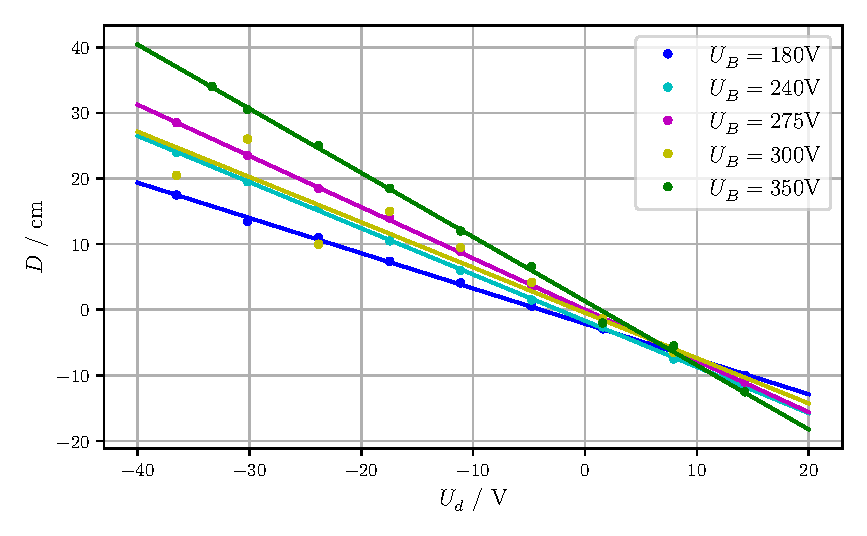
\includegraphics[width=\textwidth]{bilder/E_Feld_Teil_1.pdf}
    \caption{Die aufgenommenen Messwerte und die dazugehörigen Ausgleichsrechnungen.}
    \label{fig:eFeldTeil1a}
\end{figure}

\begin{figure} 
    \centering
    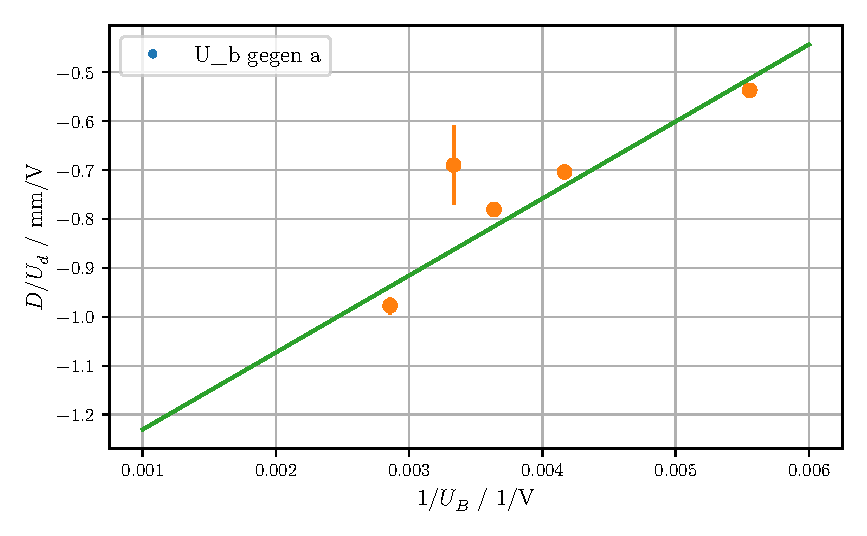
\includegraphics[width=\textwidth]{bilder/E_Feld_Teil_1_2.pdf}
    \caption{Die aufgenommenen Messwerte und die dazugehörigen Ausgleichsrechnungen.}
    \label{fig:eFeldTeil1b}
\end{figure}

Das Kathodenstrahl-Oszilloskop wird nachgebaut und verschiedene Sägezahnfrequenzen werden durchlaufen, um die Frequenz der Sinuspannung zu ermittlen.
Die aufgenommenen Messwerte sind in \autoref{tab:frequenzen} zu finden.
Das Messpaar $\sfrac{3}{2}$ und $\nu_\text{Sä} = \SI{75}{\hertz}$ wird bei der weiteren Betrachtung vernachlässigt, da dieser nicht zu dem Verhältnis passt.
Mithilfe von Gleichung \eqref{eqn:frequenzen} wird für die Sinusfrequenz $\nu_\text{Sin} = \SI{50}{\hertz}$ bestimmt, da sich aus den Messpaaren folgender Zusammenhang ergibt:
\begin{align*}
    n_1 \cdot \nu_1 &= 2 \cdot \SI{25}{\hertz} = \SI{50}{\hertz}, \\
    n_2 \cdot \nu_2 &= 1 \cdot \SI{50}{\hertz} = \SI{50}{\hertz}, \\
    n_4 \cdot \nu_4 &=  \frac{1}{2} \cdot \SI{100}{\hertz} = \SI{50}{\hertz}.
\end{align*}

\begin{table} 
    \centering
    \caption{Die aufgenommenen Messergebnisse. } 
    \label{tab:frequenzen}
    \begin{tabular}{S[table-format=3.0] S[table-format=2.1]}
    \toprule
    n & $\nu_\text{Sä} /\si{\hertz}$
      \midrule
      2 & 25 \\
      1 & 50 \\
      $\sfrac{3}{2}$ & 75 \\
      $\sfrac{1}{2}$ & 100 \\
      \bottomrule
    \end{tabular}
  \end{table}

\subsection{Elektronen im B-Feld}
\label{B-Feld}
In diesem Teil soll nun die spezifische Ladung $\frac{\symup{e_0}}{\symup{m_0}}$ bestimmt werden.
Die nach \autoref{sec:Durchführung} aufgenommenen Messwerte sind in \autoref{tab:bFeldTeil1}.
Diese werden in \autoref{fig:bFeldTeil1} aufgetragen, für beide Messreihen werden lineare Ausgleichsrechnungen der Form $\frac{D}{L^2 + D^2} = a \cdot B + b$ durchgeführt.
Dabei ist $L = \SI{0.143}{\metre}$ und die Flussdichte $B$ kann mithilfe der Gleichung \eqref{eqn:B} bestimmt werden.
% \begin{equation} \label{eq:B}
%     B = \symup{\mu_0} \cdot \frac{8}{\sqrt{125}} \cdot \frac{N\cdot I}{R}
% \end{equation} bestimmt werden.
Hier ist $N$ die Windungszahl, $I$ der Spulenstrom, $R$ der Spulenradius und $\symup{\mu_0}= \SI{4\pi\cdot 10^{-7}}{\volt\second\per\ampere\per\metre}$.
Die Windungszahl $N$ beträgt 20 und der Spulenradius $R$ ist $\SI{0.282}{\metre}$.
Für die Koeffizienten der Ausgleichsgeraden werden folgende Werte ermittelt:
\begin{align*}
U_b = \SI{250}{\volt}& &a &= -15,0649 \pm 0,0796\\ %%%%%%%%%%%%%%%%%%%%%%%%%%%%%%%%%%%%%%%%%%%%%%%%%%%%%%%%%%%%%%%%%%%%
                      &  &b &= 1,1955 \pm 0,0076\\ %%%%%%%%%%%%%%%%%% ist das schon richtig?
                      \\
U_b = \SI{420}{\volt}& &a &= -11,6417 \pm 0,1543\\
                   & &b &= -1,2456 \pm 0,0195\\
\end{align*}
Durch einen Vergleich mit der Gleichung \eqref{eq:e0_m0} ergibt sich jeweils für die spezifische Ladung:
\begin{align*}
    U_b = \SI{250}{\volt}& &\frac{\symup{e_0}}{\symup{m_0}} &= (4.5390\pm 0.0015) \cdot 10^{11} \si{\coulomb\per\kilo\gram}\\
                      \\
U_b = \SI{420}{\volt}& &\frac{\symup{e_0}}{\symup{m_0}} &= (2.7106\pm 0.0023) \cdot 10^{11} \si{\coulomb\per\kilo\gram}
\end{align*}
Daraus ergibt sich als Mittelwert für $\frac{\symup{e_0}}{\symup{m_0}} = (3.6248\pm 0.0014)\cdot 10^{11} \si{\coulomb\per\kilo\gram}$.

\begin{table} 
    \centering
    \caption{Die aufgenommenen Messergebnisse. } 
    \label{tab:bFeldTeil1}
    \begin{tabular}{S[table-format=3.0] S[table-format=2.1]}
    \toprule
        & $U_\text{b} = \SI{250}{\volt}$ & $U_\text{b} = \SI{420}{\volt}$\\
    \toprule
    $ D / \SI{6.35}{\milli\metre}$ & $I /\si{\ampere} $ \\
      \midrule
      4.0 & 0.0 & -3.25 \\
      3.0 & 0.3 & -2.95 \\
      2.0 & 0.6 & -2.5 \\
      1.0 & 0.9 & -2.1 \\
      0.0 & 1.25 & -1.65 \\
      -1.0 & 1.55 & -1.3 \\
      -2.0 & 1.9 & -0.9 \\
      -3.0 & 2.2 & -0.45 \\
      -4.0 & 2.5 & 0.0 \\
      \bottomrule
    \end{tabular}
  \end{table}

  \begin{figure} 
    \centering
    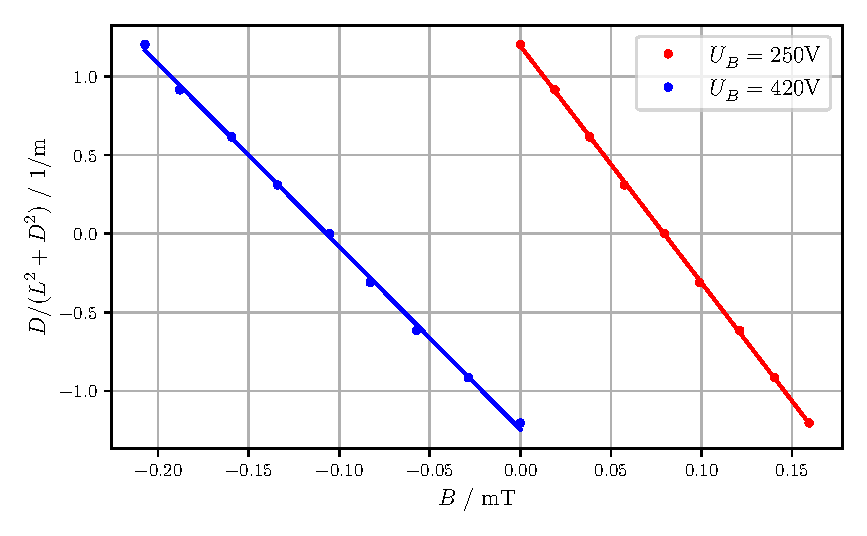
\includegraphics[width=\textwidth]{bilder/B_Feld_Teil_1_beide.pdf}
    \caption{Die aufgenommenen Messwerte und die dazugehörigen Ausgleichsrechnungen.}
    \label{fig:bFeldTeil1}
\end{figure}

Nun soll das Erdmagnetfeld bestimmt werden. Wie in \autoref{sec:Durchführung} beschrieben, wird folgender Messwert notiert:
\begin{align*}
    U_b = \SI{180}{\volt}& &I= \SI{0.55}{\ampere}.
\end{align*}
Mit der Gleichung \eqref{eq:B} kann dann das Erdmagnetfeld ermittelt werden:
\begin{align*}
    B = \SI{3.5074 \cdot 10^{-5}}{\tesla}.
\end{align*}